\FloatBarrier
\chapter{طراحی آزمایشات}

\section{آماده سازی}
شبیه سازی های آورده شده در این قسمت با استفاده از زبان برنامه پایتون
\LTRfootnote{python}
پیاده سازی شده است. از این رو چه در بخش های کار با داده و آماده سازی دادگان و چه در بخش های پردازش نیاز به دانلود و نصب برخی پکیج های مورد نیاز است. این موارد را به راحتی به کمک ابزار \texttt{pip}
می‌توان نصب کرد. برای این کار ابتدا یک فایل به نام \texttt{requirements.txt}
ایجاد کرده و داخل آن موارد نصبی را می‌نویسیم.


\begin{latin}
\begin{wgetlisting}{requirements.txt}
folium==0.2.1
numpy
tensorflow>=2.3.0
ismrmrd
sigpy
mpi4py
mridata
wget
git+git://github.com/ismrmrd/ismrmrd-python-tools.git
\end{wgetlisting}
\end{latin}

برای نصب نیز کافیست که دستور زیر را در مسیر فایل \texttt{requirements.txt} اجرا کرد.

\begin{latin}%$\bashnumbering$
\begin{lstlisting}[language=bash, frame=none, mathescape=true]
pip install -r requirements.txt 
\end{lstlisting}
\end{latin}









\section{دادگان آزمایش}
در بخش \ref{ch:background|sec:format-storage}
فرمت های گوناگون دادگان توضیح داده شد. در این آزمایش بخش مهمی از دادگان توسط سایت \urlWithoutHttp{mridata.org}
تهیه شده است. در این سایت دیتاست های خام زیادی وجود دارد که با فرمت \lr{ismrmrd}
ذخیره شده اند. همان گونه که در بخش \ref{ch:background|sec:format-storage} اشاره شد، این نوع فرمت برای ذخیره دادگان خام جهت بازسازی مناسب هستند. 




\begin{figure}[t!]
	\centering
	\copyrightbox[b]{
		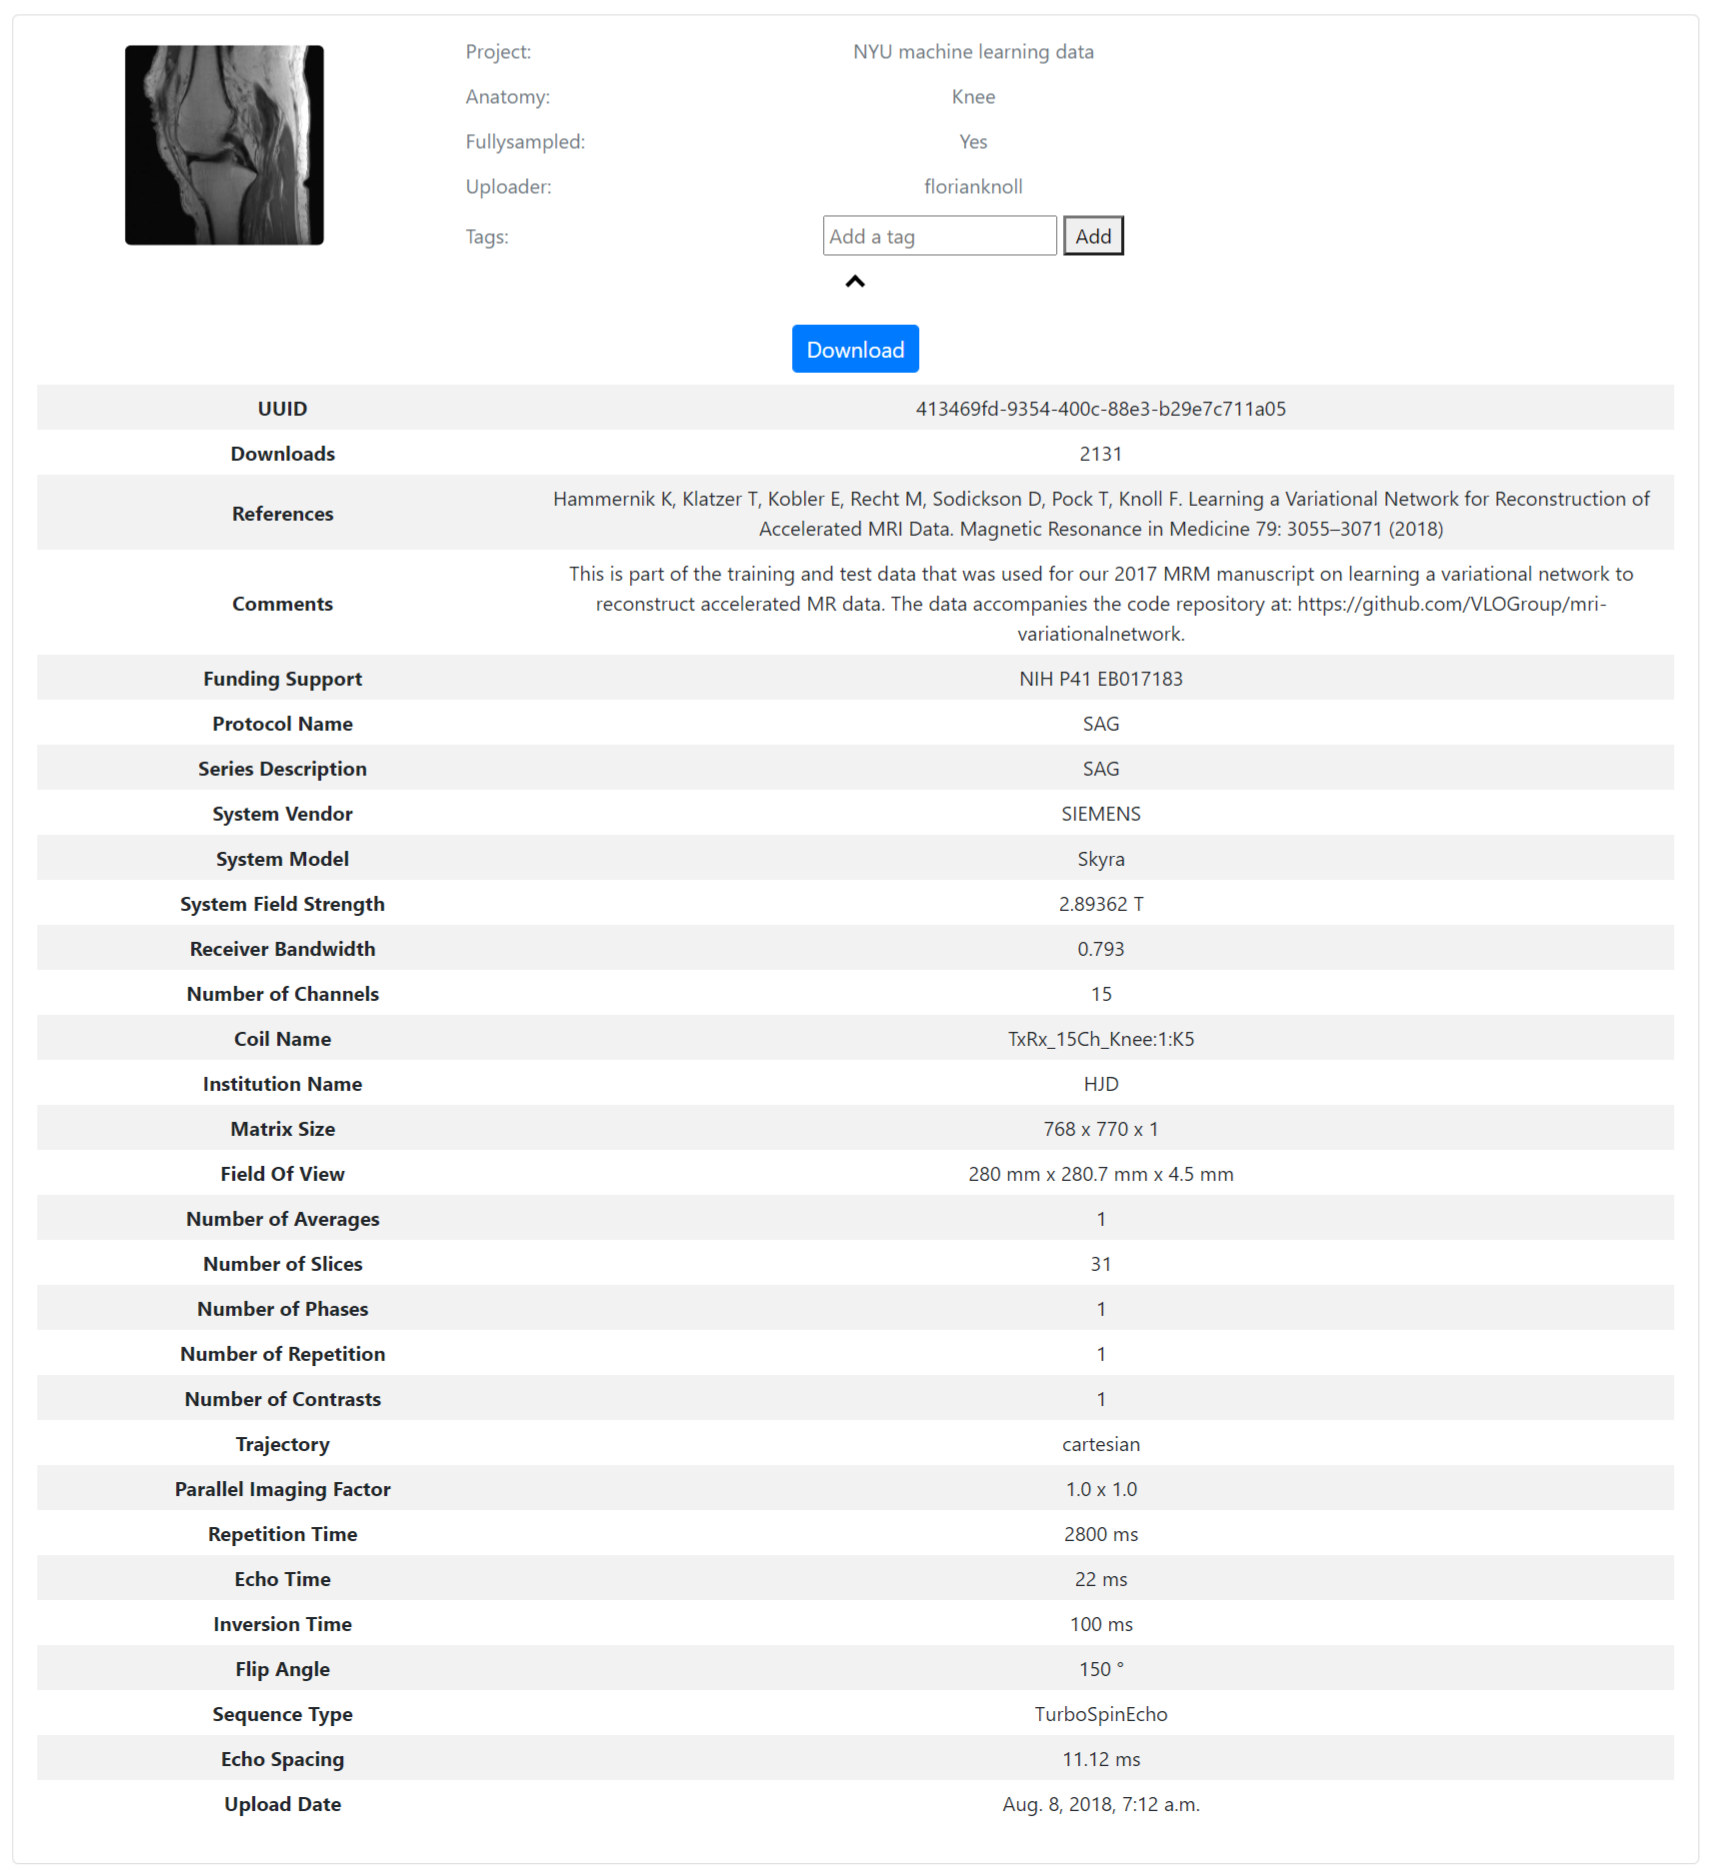
\includegraphics[width=0.9\linewidth]{chapters/chapter-4/figs/mridata-org-fields}
	}{\urlSource{http://mridata.org/list?project=NYU\%20machine\%20learning\%20data}}	
	\removevspace[1]
	\caption{}
	\label{fig:mridata-org-fields}
\end{figure}

شکل \ref{fig:mridata-org-fields}
اطلاعات مورد نیاز جهت دانلود دیتاست مورد نظر را در اختیار ما قرار می‌دهد. ردیف داده‌ی شکل \ref{fig:mridata-org-fields}، 
\lr{UUID}
آن می‌باشد که از آن جهت دانلود این دیتاست استفاده خواهیم کرد. همچنین در آن \lr{trajectory} و \lr{Parallel Imaging Factor}
به ترتیب نوع تراژکتوری اخذ داده(در اینجا کارتزین) و میزان نمونه برداری زیر نرخ (در اینجا نمونه برداری کامل انجام شده است چرا که این پارامتر یک می‌باشد.) را نشان می‌دهد.

برای استخراج جداولی مانند شکل \ref{fig:mridata-org-fields} به شکل یک لیستی از دیتافریم های کتابخانه \texttt{pandas} از کد زیر استفاده شده است:

\begin{latin}
\begin{lstlisting}
import pandas as pd
def mridataorg_to_pandas(url= 'http://mridata.org/list?project=NYU%20machine%20learning%20data'):
	tables = pd.read_html(url)
	tables = pd.concat([t.set_index(0).T for t in tables if (len(t.columns)==2 and any(t.iloc[:,0].str.contains('UUID')))])
	return tables
\end{lstlisting}
\end{latin}



\subsubsection{نحوه دانلود و خواندن داده‌ها}

برای دانلود و استفاده از دادگان این سایت در پایتون بهترین کار این است که از کد زیر استفاده کرد.


\begin{latin}
\begin{lstlisting}
import mridata, pathlib
uuid = 'cc52722b-8649-45b0-a1ea-8727c1687ad5'
dir_output = 'data'
pathlib.Path(dir_output).mkdir(parents=True, exist_ok=True)
mridata.download(uuid, folder=dir_output)
\end{lstlisting}
\end{latin}

پکیج \texttt{mridata}
برای دانلود دیتاست ها از سایت \urlWithoutHttp{mridata.org}
استفاده می‌شود و به \texttt{uuid}
دیتاست جهت انجام این کار نیاز دارد.
سپس برای خواندن این فرمت باید به شیوه زیر عمل کرد:

\begin{latin}
\begin{lstlisting}
import ismrmrd, ismrmrdtools
filename = os.path.join(dir_mridata_org, uuid+".h5")
dset = ismrmrd.Dataset(filename, 'dataset', create_if_needed=False)
header = ismrmrd.xsd.CreateFromDocument(dset.read_xml_header())
enc = header.encoding[0]
\end{lstlisting}
\end{latin}

در کد بالا پکیج \texttt{ismrmrd}
برای خواندن دادگان لازم است و پکیج \texttt{ismrmrdtools}
برای بازسازی تصاویر خام به ما کمک می‌کند. سپس سایز های ماتریس ها را می‌خوانیم.


\begin{latin}
\begin{lstlisting}
# Matrix size
eNx = enc.encodedSpace.matrixSize.x # 768
eNy = enc.encodedSpace.matrixSize.y # = 770
eNz = enc.encodedSpace.matrixSize.z # = 1
rNx = enc.reconSpace.matrixSize.x   # = 384
rNy = enc.reconSpace.matrixSize.y   # = 384
rNz = enc.reconSpace.matrixSize.z   # = 1
\end{lstlisting}
\end{latin}

با مقایسه‌ی این اندازه ماتریس فضای کد شده با ماتریس فضای باز سازی می‌توان دید که در جهت $x$ و جهت $y$ با دو برابر نرخ، نمونه برداری شده است که به اطلاح اورسمپلینگ 
\LTRfootnote{over sampling}
نامیده می‌شود.	سپس اندازه میدان دید را در این دو فضا برحسب میلی متر بدست می‌آوریم. در این صورت می‌توانیم ابعاد واقعی تصویر را مشخص کنیم.

\begin{latin}
\begin{lstlisting}
# Field of View 
eFOVx = enc.encodedSpace.fieldOfView_mm.x # = 280.0
eFOVy = enc.encodedSpace.fieldOfView_mm.y # = 280.700012
eFOVz = enc.encodedSpace.fieldOfView_mm.z # = 4.5
rFOVx = enc.reconSpace.fieldOfView_mm.x   # = 140.0 
rFOVy = enc.reconSpace.fieldOfView_mm.y   # = 140.0
rFOVz = enc.reconSpace.fieldOfView_mm.z   # = 3.0
\end{lstlisting}
\end{latin}
و برای بدست آوردن سایر اطلاعات مفید مانند تعداد اسلایس ها، تکرار ها و کنتراست از کد زیر استفاده می‌کنیم.

\begin{latin}
\begin{lstlisting}
# Number of Slices, Reps, Contrasts, etc.
ncoils = header.acquisitionSystemInformation.receiverChannels # = 15
if enc.encodingLimits.slice != None:
	nslices = enc.encodingLimits.slice.maximum + 1 # = 36
else:
	nslices = 1
if enc.encodingLimits.repetition != None:
	nreps = enc.encodingLimits.repetition.maximum + 1 # = 1
else:
	nreps = 1
if enc.encodingLimits.contrast != None:
	ncontrasts = enc.encodingLimits.contrast.maximum + 1 # = 1
else:
	ncontrasts = 1
\end{lstlisting}
\end{latin}

\subsubsection{نحوه بازسازی تصویر از داده خام}
داده های ارایه شده توسط سایت \urlWithoutHttp{mridata.org}
به صورت خام در فضای \kspace و به فرمت فایل \lr{ismrmrd}
ذخیره شده است.از آنجایی که داده ها نمونه برداری کامل شده اند، نحوه بازسازی به اطلاعات بخش \ref{ch:background}
باز می‌گردد اما از آنجا که کار با این فرمت نیز به همان اندازه پیچیده است، در این قسمت مروری بر نحوه بازساری با استفاده از پایتون خواهد شد. 

\begin{latin}
\begin{lstlisting}
import os
import ismrmrd, ismrmrd.xsd
import numpy as np
from ismrmrdtools import show, transform

# Initialiaze a storage array
all_data = np.zeros((nreps, ncontrasts, nslices, ncoils, eNz, eNy, rNx), dtype=np.complex64)

# Loop through the rest of the acquisitions and stuff
for acqnum in range(firstacq,dset.number_of_acquisitions()):
	acq = dset.read_acquisition(acqnum)
	# TODO: this is where we would apply noise pre-whitening
	# Remove oversampling if needed
	if eNx != rNx:
		xline = transform.transform_kspace_to_image(acq.data, [1])
		x0 = (eNx - rNx) // 2
		x1 = (eNx - rNx) // 2 + rNx
		xline = xline[:,x0:x1]
		acq.resize(rNx,acq.active_channels,acq.trajectory_dimensions)
		acq.center_sample = rNx//2
		# need to use the [:] notation here to fill the data
		acq.data[:] = transform.transform_image_to_kspace(xline, [1])
	# Stuff into the buffer
	rep = acq.idx.repetition
	contrast = acq.idx.contrast
	slice = acq.idx.slice
	y = acq.idx.kspace_encode_step_1
	z = acq.idx.kspace_encode_step_2
	all_data[rep, contrast, slice, :, z, y, :] = acq.data
\end{lstlisting}
\end{latin}




\begin{latin}
\begin{lstlisting}
import os
import ismrmrd
import ismrmrd.xsd
import numpy as np
import matplotlib.pyplot as plt
from ismrmrdtools import show, transform

# Initialiaze a storage array
all_data = np.zeros((nreps, ncontrasts, nslices, ncoils, eNz, eNy, eNx), dtype=np.complex64)
fig = plt.figure()
plt.xlim([0,1]); plt.ylim([0,1]);

# Loop through the rest of the acquisitions and stuff
for acqnum in range(firstacq,dset.number_of_acquisitions()):
acq = dset.read_acquisition(acqnum)

# Stuff into the buffer
rep = acq.idx.repetition
contrast = acq.idx.contrast
slice = acq.idx.slice
y = acq.idx.kspace_encode_step_1
z = acq.idx.kspace_encode_step_2
# print(y,z)
all_data[rep, contrast, slice, :, z, y, :] = acq.data
# display.clear_output(wait=True)
# x = np.arange(100)
# y = np.sin(x + np.random.rand())
# plt.plot(x, y, '-r')
# plt.show()
\end{lstlisting}
\end{latin}




\begin{latin}
\begin{lstlisting}
# Reconstruct images
images = np.zeros((nreps, ncontrasts, nslices, eNz, eNy, rNx), dtype=np.float32)
for rep in range(nreps):
	for contrast in range(ncontrasts):
		for slice in range(nslices):
			# FFT
			if eNz>1: #3D
				im = transform.transform_kspace_to_image(all_data[rep, contrast,slice,:,:,:,:], [1,2,3])
			else: #2D
				im = transform.transform_kspace_to_image(all_data[rep, contrast,slice,:,0,:,:], [1,2])
			# Sum of squares
			im = np.sqrt(np.sum(np.abs(im) ** 2, 0))
				
			# Stuff into the output
			if eNz>1: #3D
				images[rep,contrast,slice,:,:,:] = im
			else: #2D
				images[rep,contrast,slice,0,:,:] = im
# Show an image
show.imshow(np.squeeze(images[0,0,0,:,:,:]))
\end{lstlisting}
\end{latin}


\begin{figure}[t!]
	\centering
	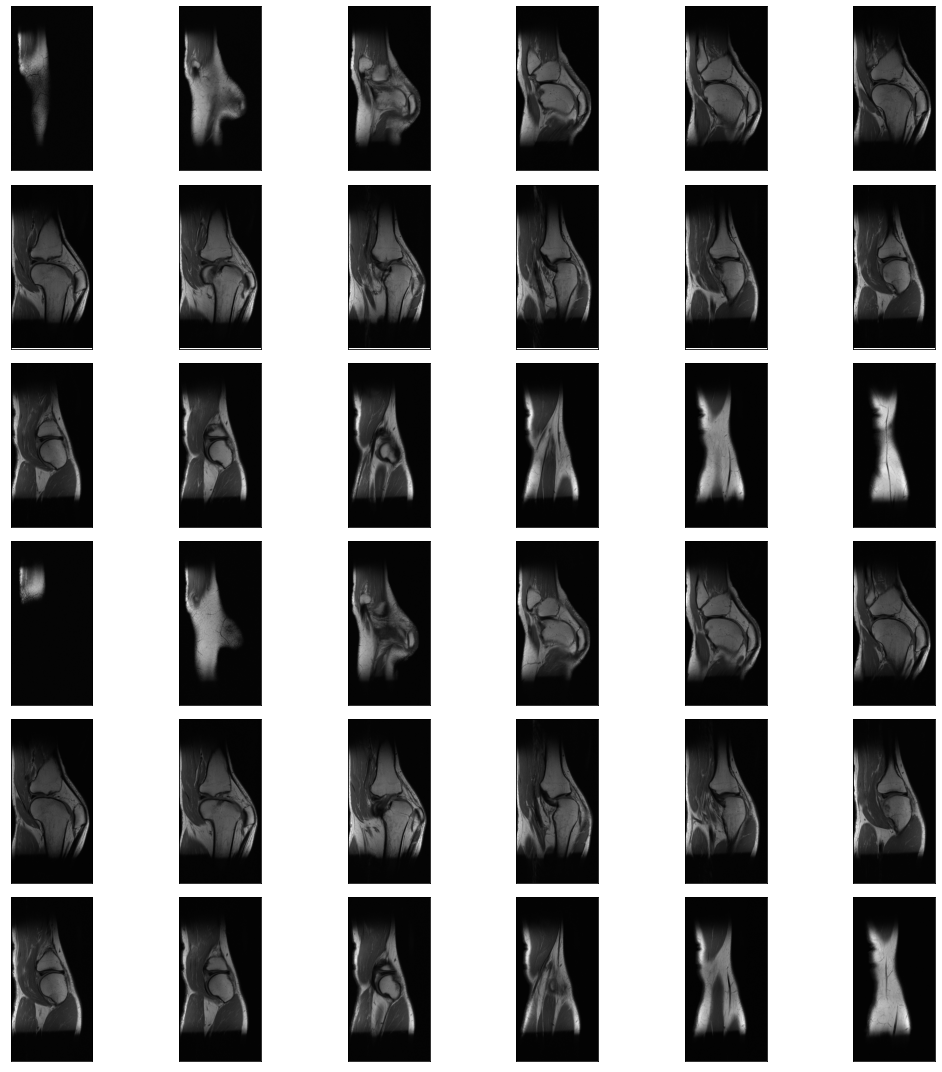
\includegraphics[width=0.7\linewidth]{chapters/chapter-4/figs/result-36-plots-data-load}
	\caption{تصاویر بازسازی شده از داده خام و نمونه برداری شده کامل}
	\label{fig:result-36-plots-data-load}
\end{figure}
